\documentclass{csse4400}

% \teachermodetrue

\usepackage{float}

\usepackage{languages}

\title{Application Programming Interfaces (APIs)}
\author{Brae Webb}

\date{\week{5}}
\begin{document}

\maketitle

\begin{figure}[h]
  \href{https://www.oreilly.com/library/view/designing-data-intensive-applications/9781491903063/ch04.html}{
    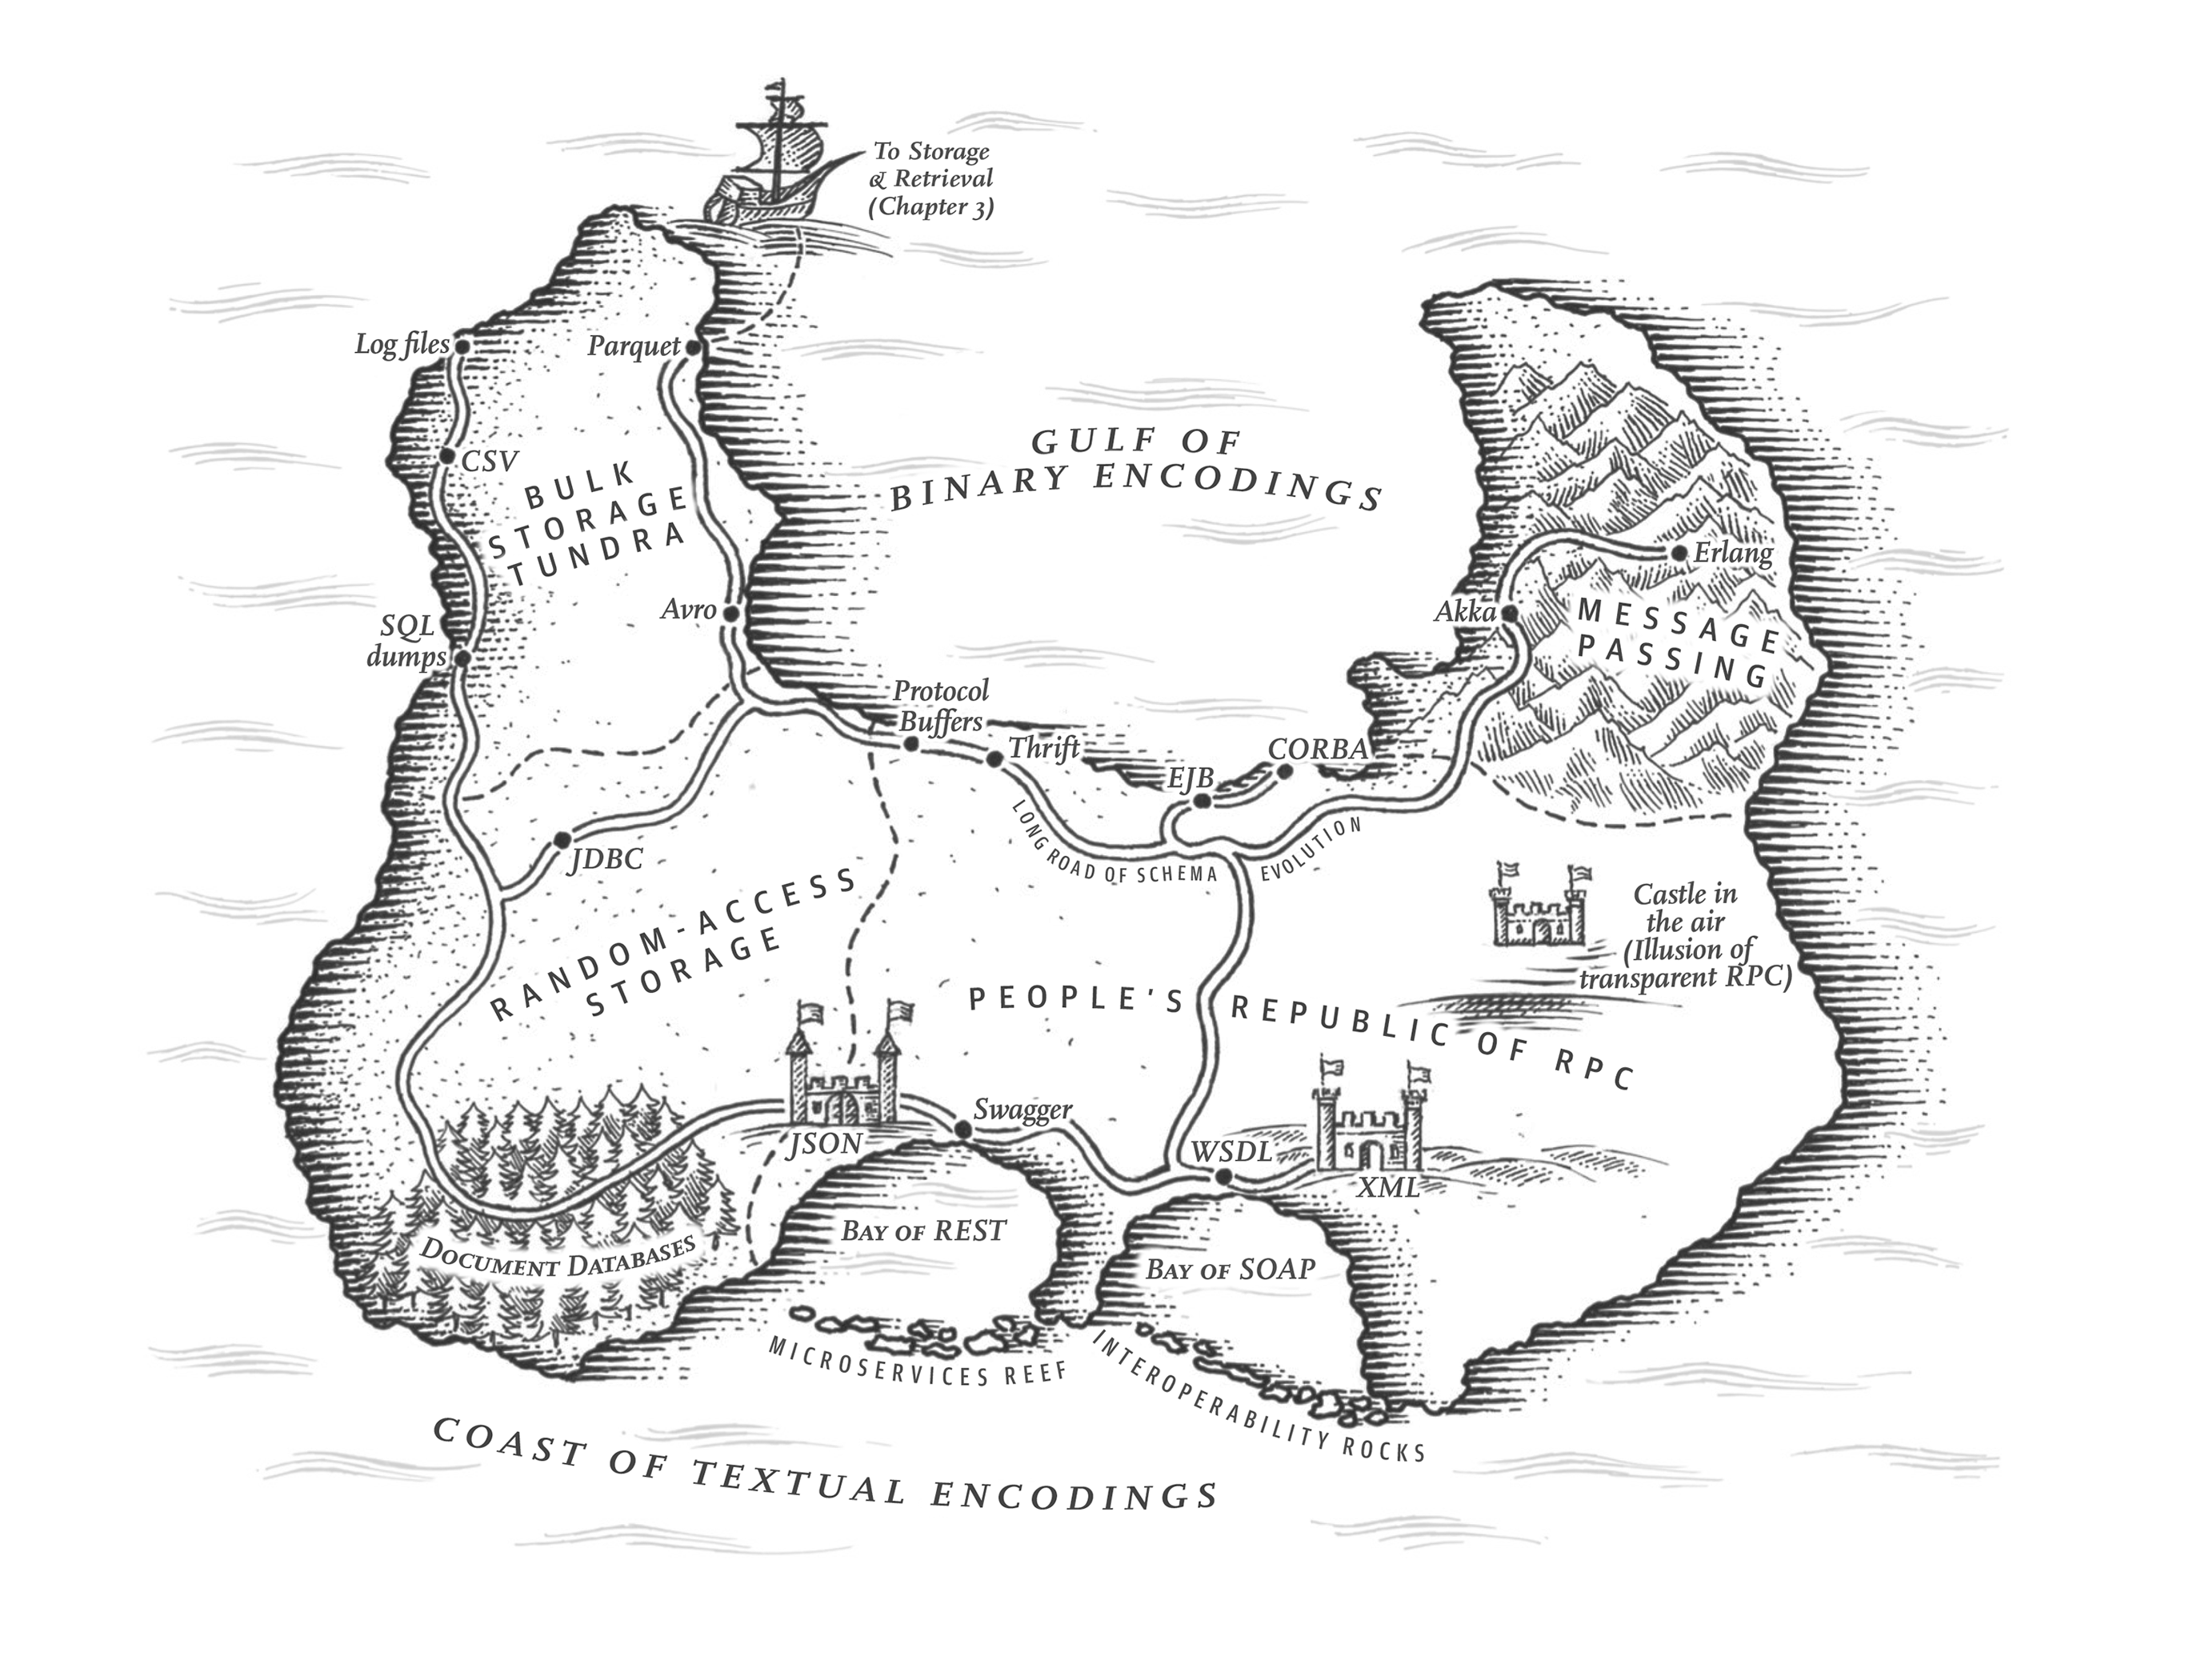
\includegraphics[width=\textwidth]{images/communication}
  }
\caption{A map of communication techniques from Designing Data-Intensive Applications \cite{data-intensive}.}
\end{figure}

\section{This Week}
This week our goal is to:
\begin{itemize}
  \item explore the various techniques developers use to communicate between components in distributed systems;
  \item finish deploying last week's todo application on AWS using terraform;
  \item use an auto-scaling group and a load balancer to increase the capacity of the todo application; and
  \item deploy the static content of the website to an S3 bucket, utilizing CloudFront to cache static content.
\end{itemize}

\teacher{
    As with last week, spend approximately the first 30 minutes exploring concepts.
}

\warning{
  \textbf{DELETE LAST WEEKS RDS INSTANCES}
}

\section{Communication}
This week we have started to explore the world of distributed systems.
The world relies (heavily) on distributed systems,
there is no machine in the world powerful enough to process the requests Google receives every second%
\footnote{Current estimates are that Google requires over a million servers}.
Even systems of a much smaller scale can still need many hundreds or thousands of machines working seamlessly together.
This inter-machine teamwork requires machines to know how to talk to each other.
For the practical this week we will look at APIs as a mechanism for communication.

\section{Data Formats}
Communication requires an exchange of information.
On computer systems information is stored at runtime in memory as primitive data which your programming language can interpret;
bytes, integers, strings, etc.
In object-oriented languages,
primitive data is wrapped up into useful packages: objects.
If we want this information to escape the confines of our programming language runtime,
we need to package it up in a language-independent format.
For a format to be language-independent we just need many languages to implement an encoding and decoding mechanism for the format.
We have a number of language-independent formats available but a few defacto standards.

\subsection{XML}
Extensible Markup Language (XML) is one of the most widely used language-independent formats.
The use cases of XML are extensive,
it's the \link{foundation for many popular utilities}{https://en.wikipedia.org/wiki/List_of_XML_markup_languages},
such as SVG file formats, SAML authentication, RSS feeds, and ePub books.

\begin{code}[language=xml]{csse6400.xml}
<root>
  <item>
    <key>Course Code</key>
    <value>CSSE6400</value>
  </item>
  <item>
    <key>Course Title</key>
    <value>Software Architecture</value>
  </item>
</root>
\end{code}

XML is designed as a markup language, similar to HTML,
it is not designed as a data exchange format.
Developers have come to point out that the verbosity and complexity of XML,
compared to alternatives such as JSON, are deal breakers.
While XML can be used as a data exchange format it is not designed for it,
and as a result APIs built around XML as a data format are becoming less common.

\subsection{JSON}
JavaScript Object Notation (JSON) is quickly replacing XML as the data format used in APIs.
As you will note, it is more succinct and communicates the important points to a human reader better.
The popularity of JSON is largely due to its compatibility with JavaScript which has taken over web development.
JSON is the map-esque data type in JavaScript.
Detractors of JSON claim that its main disadvantage compared to XML is that it lacks a schema.
However, \link{schemas are possible in JSON}{https://json-schema.org/},
they are optional, just as in XML, but are used much less than in XML.

\begin{code}[language=json]{csse6400.json}
{
    "Course Code": "CSSE6400",
    "Course Title": "Software Architecture"
}
\end{code}

\subsection{MessagePack}
It should not be a surprise that the JSON and XML formats are not resource efficient.
Nowadays, we are less concerned with squeezing data into a tiny amount of data on the hard drive as our hard drives are massive.
However, we are often concerned with how much data is being transmitted via network communication.

In the example JSON snippet above, we use 78 bytes to encode the message.
\link{MessagePack}{https://msgpack.org/} is a standard for encoding and decoding JSON.
When encoding our original JSON snippet with MessagePack we shrink to just 57 bytes.
At our scale, a negligible difference,
but at the scale of terrabytes or petabytes,
a significant consideration.

\begin{code}[]{csse6400.msgpack}
82 ab 43 6f 75 72 73 65 20 43 6f 64 65 a8 43 53 53 45 36 34 30 30 ac 43 6f 75 72 73 65 20 54 69 74 6c 65 b5 53 6f 66 74 77 61 72 65 20 41 72 63 68 69 74 65 63 74 75 72 65
\end{code}

\info{
    For those interested,
    0x82 specifies a map type (0x80) with two fields (0x02).
    Followed by a string type (0xa0) of size eleven (0x0b).
    The rest is left as an exercise: \url{https://github.com/msgpack/msgpack/blob/master/spec.md}.
}

\subsection{Protobuf}
Protocol Buffers (protobuf) is another type of binary encoding.
However, unlike MessagePack, the format was designed from scratch,
allowing a more compact and better designed format.
Protobufs require all data to be defined by a schema.
For example:

\begin{code}[language=protobuf]{csse6400.proto}
message Course {
    required string code = 1;
    required string name = 2;
}
\end{code}

Protobufs differ from XML, JSON, and MessagePack via their method of integration.
In the previous examples,
your language would have a library to encode and decode the data format into and out of your language's type system.
With protobuf, an external tool, \textsl{protoc},
takes the schema and generates a model of the schema in your target language.
This gives every language a native method to interact with the data format,
it often means that developers do not need to be aware of the underlying encoding.

\begin{code}[language=java]{csse6400.java}
Course softarch = Course.newBuilder()
    .setCode("CSSE6400")
    .setName("Software Architecture")
    .build();
output = new FileOutputStream(args[0]);
softarch.writeTo(output);
\end{code}

\section{Application Programming Interfaces}
It is worth being aware of a few of the common API paradigms available.
We outline a few but note that in this course we will primarily focus on REST APIs.
This is only an indication that they are better understood by course staff,
not their superiority.

\subsection{XML-RPC}
XML-RPC was one of the first API standards.
It is a Remote Procedure Call (RPC) based API which communicates via XML.
It is not a commonly used standard anymore.

\subsection{SOAP}
After XML-RPC came SOAP.
SOAP was impactful for service-oriented (now microservice) architectures but has largely fallen out of favor in-place of REST APIs.
We do not cover SOAP in any meaningful depth due to it's increasing irrelevance and complexity.

\subsection{REST}
REST is not a standard like SOAP once was,
instead REST is an architectural style guided by a set of architectural constraints that allows us to build flexible APIs.

In this course we do not dive too deep into the architectural style and instead opt for a more surface level understanding.
It is a common mistake for people to refer to REST as a HTTP based web service API,
they are different.
In this course we chose to embrace this mistake and often refer to a HTTP based web service API when saying REST.

\noindent An example of this type of API might be:
\begin{description}
  \item[GET /api/v1/todo] List all tasks todo
  \item[POST /api/v1/todo] Create a task todo
  \item[GET /api/v1/todo/{id}] List all details about a certain task
  \item[PUT /api/v1/todo/{id}] Update the fields of an existing task
  \item[DELETE /api/v1/todo/{id}] Delete a specific task
\end{description}

\subsection{JSON-RPC}
A JSON RPC is another RPC based API based around communication via JSON.
When deciding whether to use an RPC-based API or a REST/SOAP based API,
the common distinction to make is that RPC APIs should be action based, i.e. I want to do X.
Whereas REST/SOAP APIs are Create Read Update Delete (CRUD) based for providing a interface to mutable data.

\subsection{GraphQL}
GraphQL is a query language which allows more dynamic querying of data than REST based APIs.
You can create nested queries and specify the fields you want to receive in response.
GraphQL APIs are well-suited for building APIs designed for developers to consume but when dealing with rigid inter-service based request,
REST APIs are generally preferable.

\subsection{gRPC}
Another RPC framework, gRPC has started gaining a lot of attention since its first release in 2016.
gRPC is based on protobuf communication standard.
In addition to a more type-safe system,
gRPC based APIs provide authentication and streaming mechanisms.

\section{Deploying a Todo Part Two}

In the practical last week we deployed a very simple todo application.
Recall that we deployed a MySQL database on RDS and an EC2 instance which acted as a Docker container.
The Docker container connected to the database and handled CRUD requests via a REST API.
The Docker container was also responsible for serving static content.
In this practical, we will explore two approaches to better scale our application.
We assume that you have last weeks practical setup in Terraform, if not, do that now.

\warning{
  The Docker image from last week has moved to
  
  \texttt{ghcr.io/csse6400/todo-app:combined-latest}
}

\subsection{Scaling EC2}
As we've now seen in the lectures,
cloud platforms such as AWS offer useful techniques for scaling our systems.
Our first task for the practical will be to use an auto-scaling group and a load balancer to double our compute capacity.
Our desired deployment diagram is shown in Figure \ref{fig:scale}.

\begin{figure}[ht]
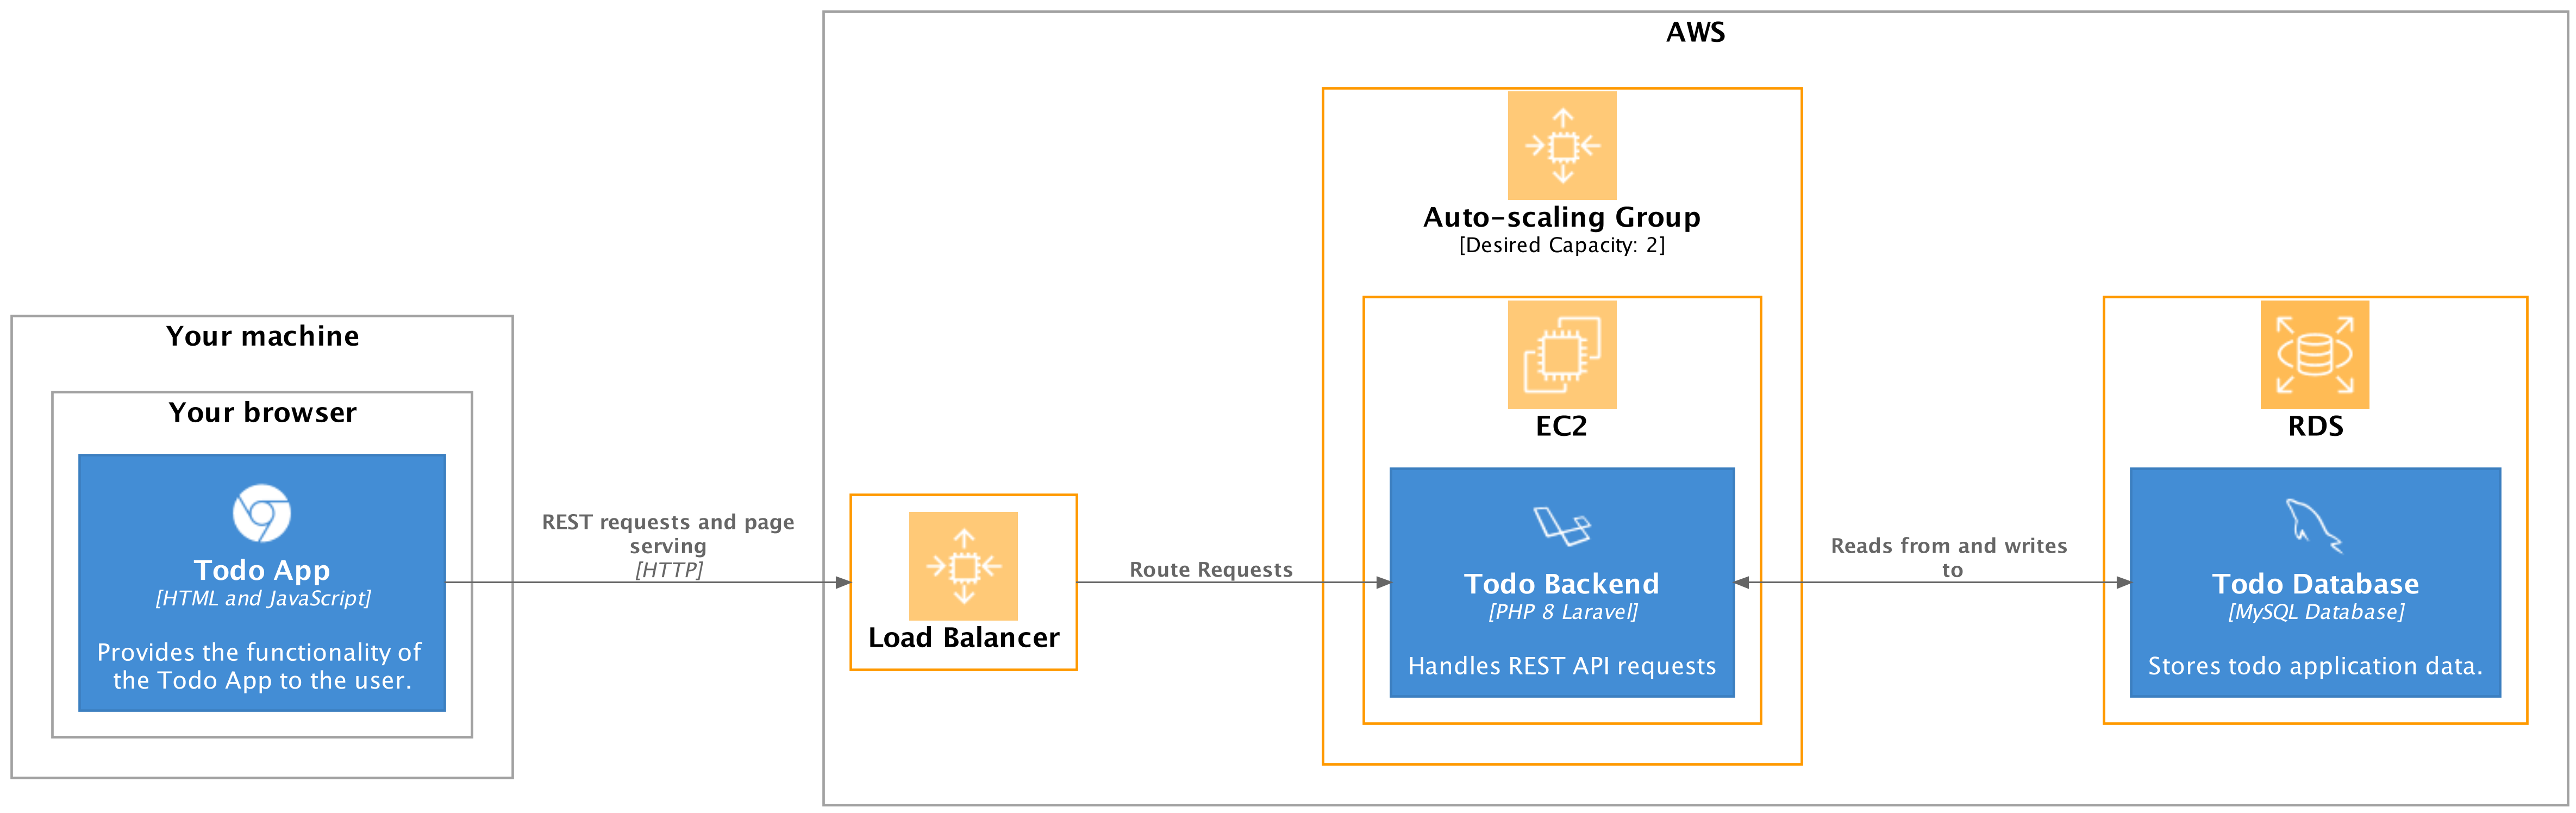
\includegraphics[width=\textwidth]{diagrams/ScaleDeployment}
\caption{Desired deployment diagram of the todo application using auto-scaling and a load balancer.}
\label{fig:scale}
\end{figure}

In order to give you practice developing Terraform independently,
we will not distribute Terraform configuration for this exercise.
Instead we will provide an outline of what is required with links as appropriate.

\begin{enumerate}
  \item We need to tell the auto-scaling group how to create new instances.
  We will want to use \link{launch templates}{https://registry.terraform.io/providers/hashicorp/aws/latest/docs/resources/launch_template}.
  \info{
    You may find this module helpful: \url{https://github.com/CSSE6400/terraform/tree/main/template}.
    It creates a launch template based on a Docker image similar to the custom module last week.
    Note that the security group list will need to specify security group ids rather than security group names as in the previous module.
  }
  \item We need an \link{auto-scaling group}{https://registry.terraform.io/providers/hashicorp/aws/latest/docs/resources/autoscaling_group} with a desired capacity of two.
  \item We need a \link{load balancer}{https://registry.terraform.io/providers/hashicorp/aws/latest/docs/resources/lb}.
  A load balancer needs to be in subnets in at least two different availability zones.
  A list of all subnets in the default VPC can be created using the following:
  \begin{code}[language=terraform]{}
data "aws_subnet_ids" "nets" {
  vpc_id = aws_security_group.todoapp-backend.vpc_id
}
  \end{code}
  \warning{Do not forget to attach an appropriate security group to the load balancer.}
  \item We need a \link{load balancer target group}{https://registry.terraform.io/providers/hashicorp/aws/latest/docs/resources/lb_target_group}.
  \item We need a \link{load balancer listener}{https://registry.terraform.io/providers/hashicorp/aws/latest/docs/resources/lb_listener} to direct traffic to our load balancer target group.
  \item Finally, we can use an \link{auto-scaling attachment}{https://registry.terraform.io/providers/hashicorp/aws/latest/docs/resources/autoscaling_attachment} to attach our load balancer target group to our auto-scaling group.
\end{enumerate}

\subsection{Distributing Static Serving \& Caching}

\info{
  This section will gradually offer less guidance,
  eventually leaving you to discover the final implementation completely independently.
  We recommend that you try and get as far as you can on your own and ask a tutor when stuck.
  It is important that you can deploy AWS resources via Terraform unassisted for the assignment (and your future careers).
}

The EC2 instance is responsible for:
\begin{enumerate}
  \item allowing users to download the client-side HTML and Javascript frontend; and
  \item providing a REST API the client talked to in order to access persistent data.
\end{enumerate}
This means that each time the client opens the website they will need to download the frontend and make all subsequent requests to the same instance.
This does not scale well.

The todo application was built using a simple layered architecture.
\begin{enumerate}
  \item The client-side (or presentation layer) is developed in \link{Elm}{https://elm-lang.org/} which compiles into static HTML and JavaScript.
  \item The presentation layer communicates with a \link{Laravel}{https://laravel.com/} persistence layer via a REST API.
  \item The persistence layer in turn communicates with a \link{MySQL}{https://www.mysql.com/} database layer.
\end{enumerate}

We have already deployed the database layer separately from the presentation and persistence layer.
Now, we want to deploy the service which serves the presentation layer separately from the persistence layer.
Since our presentation layer is static,
we can take advantage of the AWS S3 service.
AWS S3 is scalable, which means that we do not have to worry about manually scaling our frontend serving (and can focus on the challenge of backend scaling).

\begin{figure}[ht]
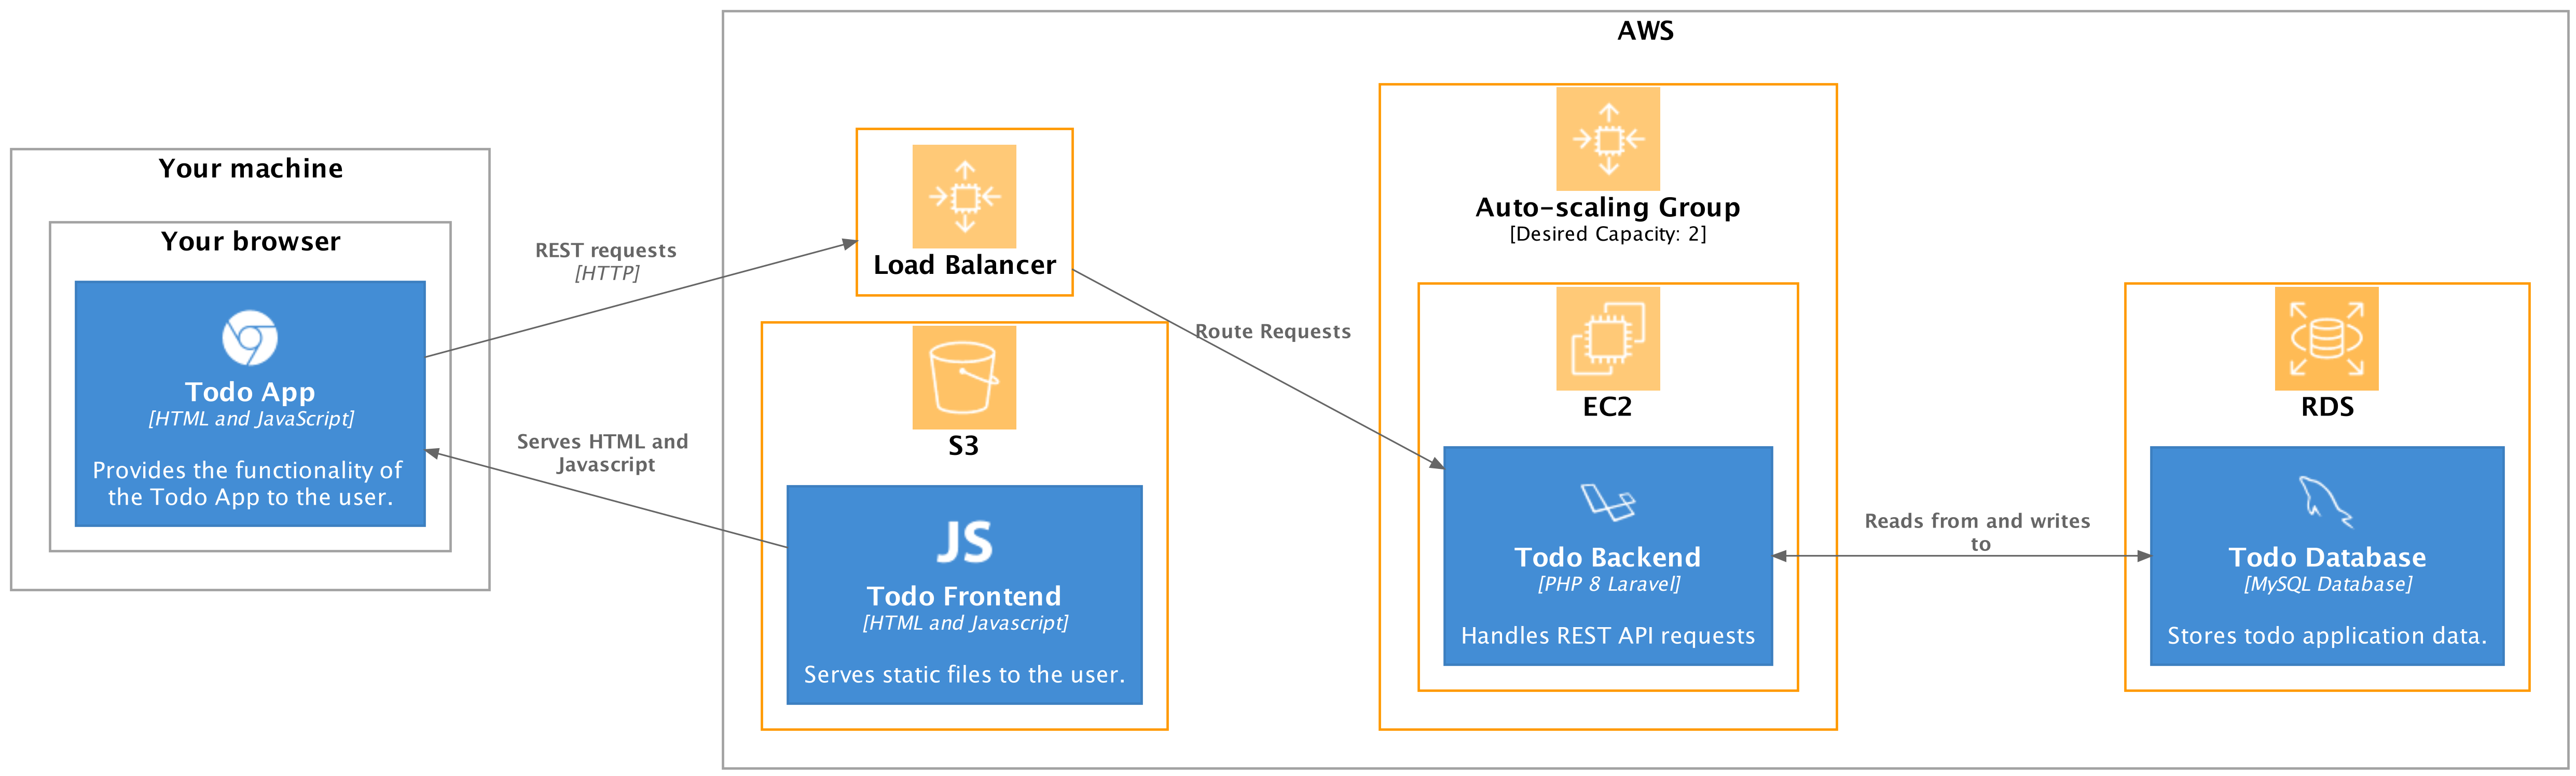
\includegraphics[width=\textwidth]{diagrams/SimpleS3Deployment}
\caption{Desired deployment diagram of the todo application.}
\end{figure}

\subsection{Deploying EC2 \& RDS}
Our current Docker image combines static serving with the REST API.
Now, we want to update the version of our EC2 instances so that it does not also serve static HTML pages.
To do this,
update your docker image to be \textsl{v0.9.1} instead of \textsl{combined-latest},
i.e. \texttt{ghcr.io/csse6400/todo-app:v0.9.1}
If you try to access this updated EC2 instance, 
you should be prompted with `Hey!, if you see this page then the ALB probably isnt working :('.

\subsection{Deploying an S3 Bucket}
We now want to deploy our static HTML to an S3 bucket.
Our single HTML file for the web application is released via GitHub releases, available here:

\noindent\texttt{https://github.com/CSSE6400/todo-app/releases/download/v0.9.1/index.html}

\noindent The following steps provide an outline for deploying the static website to S3.

\begin{enumerate}
  \item Terraform bucket names much be unique lowercase and without special characters.
  
  \url{https://registry.terraform.io/providers/hashicorp/random/latest/docs/resources/string}

  \item A bucket must be made publicly available.
  
  \url{https://registry.terraform.io/providers/hashicorp/aws/latest/docs/resources/s3_bucket_acl}

  \item Remote resources can be gathered via the \texttt{http} data source in terraform: 
  
  \url{https://registry.terraform.io/providers/hashicorp/http/latest/docs/data-sources/http}

  \item The static HTML page must be uploaded to the bucket.
  
  \url{https://registry.terraform.io/providers/hashicorp/aws/latest/docs/resources/s3_bucket_object}

  \item The uploaded HTML must be configured as a website.
  
  \url{https://registry.terraform.io/providers/hashicorp/aws/latest/docs/resources/s3_bucket_website_configuration}
\end{enumerate}

\noindent Once you are getting permission denied,
attach the policy below to allow access using \link{\texttt{s3\_bucket\_policy}}{https://registry.terraform.io/providers/hashicorp/aws/latest/docs/resources/s3_bucket_policy}

\begin{code}[language=terraform]{}
data "aws_iam_policy_document" "website_policy" {
  statement {
    actions = [
      "s3:GetObject"
    ]
    principals {
      identifiers = ["*"]
      type = "AWS"
    }
    effect = "Allow"
    resources = [
      "arn:aws:s3:::${aws_s3_bucket.frontend-bucket.id}/*"
    ]
  }
}
\end{code}

This should give you an S3 bucket which, when accessed,
will fail to connect to the backend with a 404.
This occurs because it is looking on the S3 bucket server for the backend.

One approach to this problem would be to configure the frontend to know which server to talk to for the backend.
The approach we will take is to place the EC2 instance and S3 bucket behind a CloudFront service.
This will allow them to share the same domain name and provide better caching mechanisms.
Our desired state is shown in Figure \ref{fig:s3deployment}.

\begin{figure}[ht]
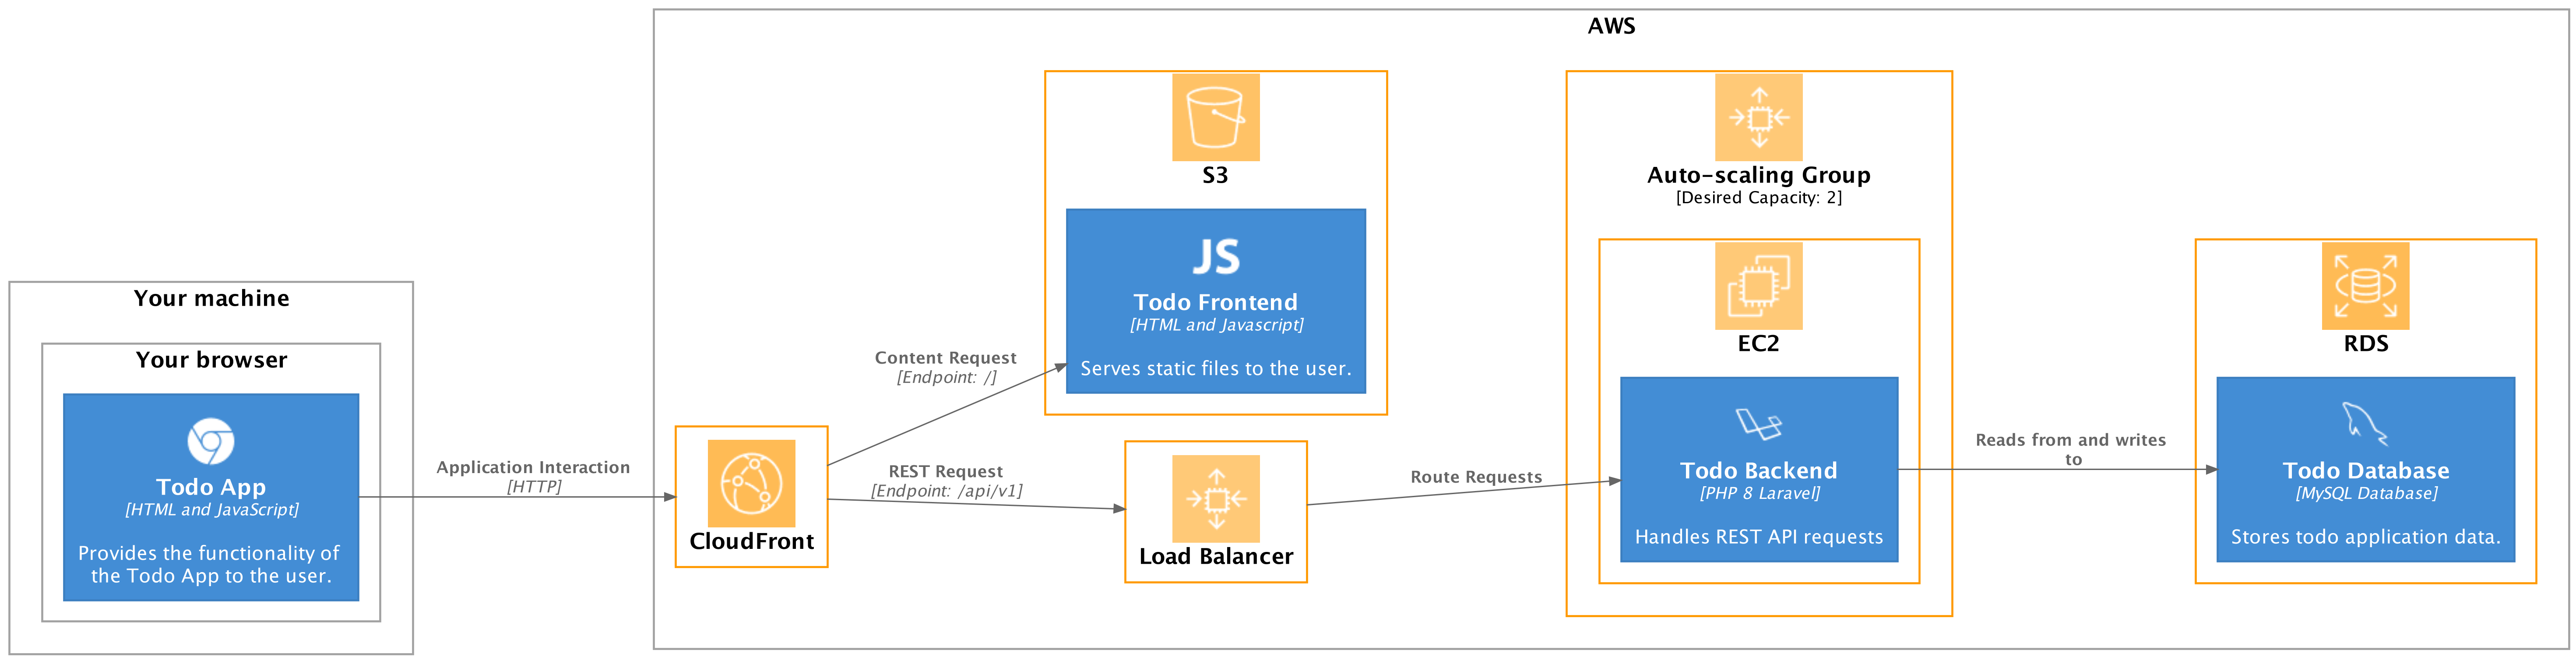
\includegraphics[width=\textwidth]{diagrams/S3Deployment}
\caption{Desired deployment diagram of the todo application using CloudFront to route requests.}
\label{fig:s3deployment}
\end{figure}

That is all from us,
the implementation of the CloudFront service in from of your S3 Bucket and Load Balancer is now up to you to discover.
This type of deep-dive into the Terraform documentation will be extremely useful for your upcoming assignment.
Best of luck!

\bibliographystyle{ieeetr}
\bibliography{books,ours}

\end{document}